\documentclass[]{book}
\usepackage{lmodern}
\usepackage{amssymb,amsmath}
\usepackage{ifxetex,ifluatex}
\usepackage{fixltx2e} % provides \textsubscript
\ifnum 0\ifxetex 1\fi\ifluatex 1\fi=0 % if pdftex
  \usepackage[T1]{fontenc}
  \usepackage[utf8]{inputenc}
\else % if luatex or xelatex
  \ifxetex
    \usepackage{mathspec}
  \else
    \usepackage{fontspec}
  \fi
  \defaultfontfeatures{Ligatures=TeX,Scale=MatchLowercase}
\fi
% use upquote if available, for straight quotes in verbatim environments
\IfFileExists{upquote.sty}{\usepackage{upquote}}{}
% use microtype if available
\IfFileExists{microtype.sty}{%
\usepackage{microtype}
\UseMicrotypeSet[protrusion]{basicmath} % disable protrusion for tt fonts
}{}
\usepackage{hyperref}
\hypersetup{unicode=true,
            pdftitle={R for the Excel User},
            pdfauthor={Julie Lowndes \& Allison Horst},
            pdfborder={0 0 0},
            breaklinks=true}
\urlstyle{same}  % don't use monospace font for urls
\usepackage{natbib}
\bibliographystyle{apalike}
\usepackage{color}
\usepackage{fancyvrb}
\newcommand{\VerbBar}{|}
\newcommand{\VERB}{\Verb[commandchars=\\\{\}]}
\DefineVerbatimEnvironment{Highlighting}{Verbatim}{commandchars=\\\{\}}
% Add ',fontsize=\small' for more characters per line
\usepackage{framed}
\definecolor{shadecolor}{RGB}{248,248,248}
\newenvironment{Shaded}{\begin{snugshade}}{\end{snugshade}}
\newcommand{\AlertTok}[1]{\textcolor[rgb]{0.94,0.16,0.16}{#1}}
\newcommand{\AnnotationTok}[1]{\textcolor[rgb]{0.56,0.35,0.01}{\textbf{\textit{#1}}}}
\newcommand{\AttributeTok}[1]{\textcolor[rgb]{0.77,0.63,0.00}{#1}}
\newcommand{\BaseNTok}[1]{\textcolor[rgb]{0.00,0.00,0.81}{#1}}
\newcommand{\BuiltInTok}[1]{#1}
\newcommand{\CharTok}[1]{\textcolor[rgb]{0.31,0.60,0.02}{#1}}
\newcommand{\CommentTok}[1]{\textcolor[rgb]{0.56,0.35,0.01}{\textit{#1}}}
\newcommand{\CommentVarTok}[1]{\textcolor[rgb]{0.56,0.35,0.01}{\textbf{\textit{#1}}}}
\newcommand{\ConstantTok}[1]{\textcolor[rgb]{0.00,0.00,0.00}{#1}}
\newcommand{\ControlFlowTok}[1]{\textcolor[rgb]{0.13,0.29,0.53}{\textbf{#1}}}
\newcommand{\DataTypeTok}[1]{\textcolor[rgb]{0.13,0.29,0.53}{#1}}
\newcommand{\DecValTok}[1]{\textcolor[rgb]{0.00,0.00,0.81}{#1}}
\newcommand{\DocumentationTok}[1]{\textcolor[rgb]{0.56,0.35,0.01}{\textbf{\textit{#1}}}}
\newcommand{\ErrorTok}[1]{\textcolor[rgb]{0.64,0.00,0.00}{\textbf{#1}}}
\newcommand{\ExtensionTok}[1]{#1}
\newcommand{\FloatTok}[1]{\textcolor[rgb]{0.00,0.00,0.81}{#1}}
\newcommand{\FunctionTok}[1]{\textcolor[rgb]{0.00,0.00,0.00}{#1}}
\newcommand{\ImportTok}[1]{#1}
\newcommand{\InformationTok}[1]{\textcolor[rgb]{0.56,0.35,0.01}{\textbf{\textit{#1}}}}
\newcommand{\KeywordTok}[1]{\textcolor[rgb]{0.13,0.29,0.53}{\textbf{#1}}}
\newcommand{\NormalTok}[1]{#1}
\newcommand{\OperatorTok}[1]{\textcolor[rgb]{0.81,0.36,0.00}{\textbf{#1}}}
\newcommand{\OtherTok}[1]{\textcolor[rgb]{0.56,0.35,0.01}{#1}}
\newcommand{\PreprocessorTok}[1]{\textcolor[rgb]{0.56,0.35,0.01}{\textit{#1}}}
\newcommand{\RegionMarkerTok}[1]{#1}
\newcommand{\SpecialCharTok}[1]{\textcolor[rgb]{0.00,0.00,0.00}{#1}}
\newcommand{\SpecialStringTok}[1]{\textcolor[rgb]{0.31,0.60,0.02}{#1}}
\newcommand{\StringTok}[1]{\textcolor[rgb]{0.31,0.60,0.02}{#1}}
\newcommand{\VariableTok}[1]{\textcolor[rgb]{0.00,0.00,0.00}{#1}}
\newcommand{\VerbatimStringTok}[1]{\textcolor[rgb]{0.31,0.60,0.02}{#1}}
\newcommand{\WarningTok}[1]{\textcolor[rgb]{0.56,0.35,0.01}{\textbf{\textit{#1}}}}
\usepackage{longtable,booktabs}
\usepackage{graphicx,grffile}
\makeatletter
\def\maxwidth{\ifdim\Gin@nat@width>\linewidth\linewidth\else\Gin@nat@width\fi}
\def\maxheight{\ifdim\Gin@nat@height>\textheight\textheight\else\Gin@nat@height\fi}
\makeatother
% Scale images if necessary, so that they will not overflow the page
% margins by default, and it is still possible to overwrite the defaults
% using explicit options in \includegraphics[width, height, ...]{}
\setkeys{Gin}{width=\maxwidth,height=\maxheight,keepaspectratio}
\IfFileExists{parskip.sty}{%
\usepackage{parskip}
}{% else
\setlength{\parindent}{0pt}
\setlength{\parskip}{6pt plus 2pt minus 1pt}
}
\setlength{\emergencystretch}{3em}  % prevent overfull lines
\providecommand{\tightlist}{%
  \setlength{\itemsep}{0pt}\setlength{\parskip}{0pt}}
\setcounter{secnumdepth}{5}
% Redefines (sub)paragraphs to behave more like sections
\ifx\paragraph\undefined\else
\let\oldparagraph\paragraph
\renewcommand{\paragraph}[1]{\oldparagraph{#1}\mbox{}}
\fi
\ifx\subparagraph\undefined\else
\let\oldsubparagraph\subparagraph
\renewcommand{\subparagraph}[1]{\oldsubparagraph{#1}\mbox{}}
\fi

%%% Use protect on footnotes to avoid problems with footnotes in titles
\let\rmarkdownfootnote\footnote%
\def\footnote{\protect\rmarkdownfootnote}

%%% Change title format to be more compact
\usepackage{titling}

% Create subtitle command for use in maketitle
\providecommand{\subtitle}[1]{
  \posttitle{
    \begin{center}\large#1\end{center}
    }
}

\setlength{\droptitle}{-2em}

  \title{R for the Excel User}
    \pretitle{\vspace{\droptitle}\centering\huge}
  \posttitle{\par}
    \author{Julie Lowndes \& Allison Horst}
    \preauthor{\centering\large\emph}
  \postauthor{\par}
      \predate{\centering\large\emph}
  \postdate{\par}
    \date{2019-08-17}

\usepackage{booktabs}

\begin{document}
\maketitle

{
\setcounter{tocdepth}{1}
\tableofcontents
}
\hypertarget{prerequisites}{%
\chapter{Prerequisites}\label{prerequisites}}

This is a \emph{sample} book written in \textbf{Markdown}. You can use anything that Pandoc's Markdown supports, e.g., a math equation \(a^2 + b^2 = c^2\).

The \textbf{bookdown} package can be installed from CRAN or Github:

\begin{Shaded}
\begin{Highlighting}[]
\KeywordTok{install.packages}\NormalTok{(}\StringTok{"bookdown"}\NormalTok{)}
\CommentTok{# or the development version}
\CommentTok{# devtools::install_github("rstudio/bookdown")}
\end{Highlighting}
\end{Shaded}

Remember each Rmd file contains one and only one chapter, and a chapter is defined by the first-level heading \texttt{\#}.

To compile this example to PDF, you need XeLaTeX. You are recommended to install TinyTeX (which includes XeLaTeX): \url{https://yihui.name/tinytex/}.

You can label chapter and section titles using \texttt{\{\#label\}} after them, e.g., we can reference Chapter \ref{overview}. If you do not manually label them, there will be automatic labels anyway, e.g., Chapter \ref{readxl}.

Figures and tables with captions will be placed in \texttt{figure} and \texttt{table} environments, respectively.

\begin{Shaded}
\begin{Highlighting}[]
\KeywordTok{par}\NormalTok{(}\DataTypeTok{mar =} \KeywordTok{c}\NormalTok{(}\DecValTok{4}\NormalTok{, }\DecValTok{4}\NormalTok{, }\FloatTok{.1}\NormalTok{, }\FloatTok{.1}\NormalTok{))}
\KeywordTok{plot}\NormalTok{(pressure, }\DataTypeTok{type =} \StringTok{'b'}\NormalTok{, }\DataTypeTok{pch =} \DecValTok{19}\NormalTok{)}
\end{Highlighting}
\end{Shaded}

\begin{figure}

{\centering 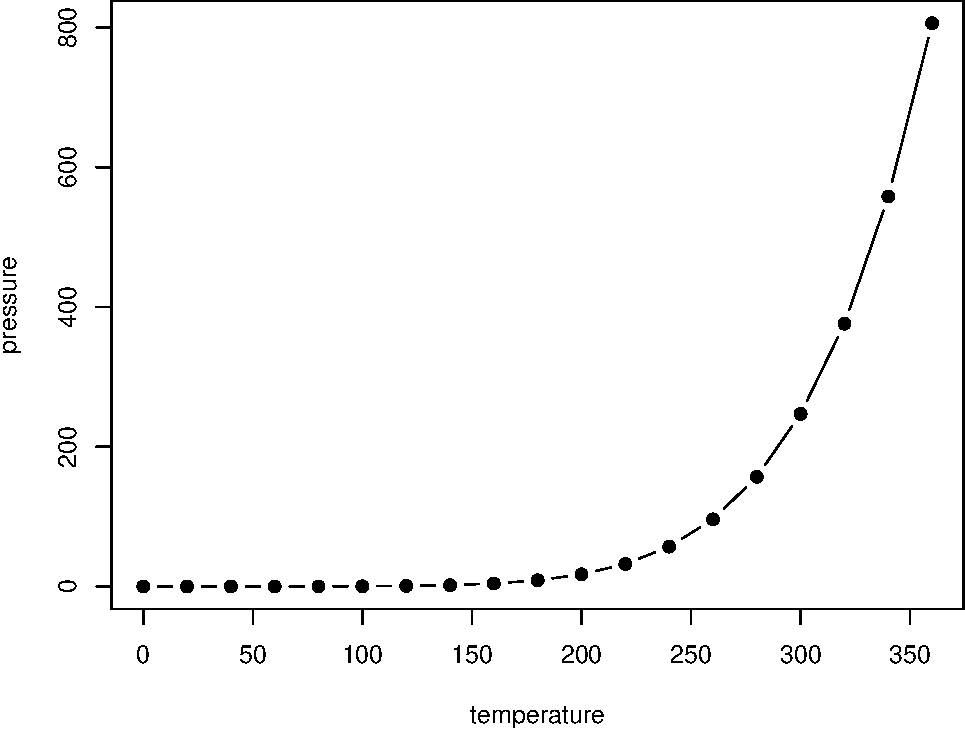
\includegraphics[width=0.8\linewidth]{R_for_Excel_Users_files/figure-latex/nice-fig-1} 

}

\caption{Here is a nice figure!}\label{fig:nice-fig}
\end{figure}

Reference a figure by its code chunk label with the \texttt{fig:} prefix, e.g., see Figure \ref{fig:nice-fig}. Similarly, you can reference tables generated from \texttt{knitr::kable()}, e.g., see Table \ref{tab:nice-tab}.

\begin{Shaded}
\begin{Highlighting}[]
\NormalTok{knitr}\OperatorTok{::}\KeywordTok{kable}\NormalTok{(}
  \KeywordTok{head}\NormalTok{(iris, }\DecValTok{20}\NormalTok{), }\DataTypeTok{caption =} \StringTok{'Here is a nice table!'}\NormalTok{,}
  \DataTypeTok{booktabs =} \OtherTok{TRUE}
\NormalTok{)}
\end{Highlighting}
\end{Shaded}

\begin{table}[t]

\caption{\label{tab:nice-tab}Here is a nice table!}
\centering
\begin{tabular}{rrrrl}
\toprule
Sepal.Length & Sepal.Width & Petal.Length & Petal.Width & Species\\
\midrule
5.1 & 3.5 & 1.4 & 0.2 & setosa\\
4.9 & 3.0 & 1.4 & 0.2 & setosa\\
4.7 & 3.2 & 1.3 & 0.2 & setosa\\
4.6 & 3.1 & 1.5 & 0.2 & setosa\\
5.0 & 3.6 & 1.4 & 0.2 & setosa\\
\addlinespace
5.4 & 3.9 & 1.7 & 0.4 & setosa\\
4.6 & 3.4 & 1.4 & 0.3 & setosa\\
5.0 & 3.4 & 1.5 & 0.2 & setosa\\
4.4 & 2.9 & 1.4 & 0.2 & setosa\\
4.9 & 3.1 & 1.5 & 0.1 & setosa\\
\addlinespace
5.4 & 3.7 & 1.5 & 0.2 & setosa\\
4.8 & 3.4 & 1.6 & 0.2 & setosa\\
4.8 & 3.0 & 1.4 & 0.1 & setosa\\
4.3 & 3.0 & 1.1 & 0.1 & setosa\\
5.8 & 4.0 & 1.2 & 0.2 & setosa\\
\addlinespace
5.7 & 4.4 & 1.5 & 0.4 & setosa\\
5.4 & 3.9 & 1.3 & 0.4 & setosa\\
5.1 & 3.5 & 1.4 & 0.3 & setosa\\
5.7 & 3.8 & 1.7 & 0.3 & setosa\\
5.1 & 3.8 & 1.5 & 0.3 & setosa\\
\bottomrule
\end{tabular}
\end{table}

You can write citations, too. For example, we are using the \textbf{bookdown} package \citep{R-bookdown} in this sample book, which was built on top of R Markdown and \textbf{knitr} \citep{xie2015}.

\hypertarget{overview}{%
\chapter{Overview}\label{overview}}

\begin{center}\rule{0.5\linewidth}{\linethickness}\end{center}

References Brainstorm

\begin{itemize}
\tightlist
\item
  Broman \& Woo 2017: \url{https://www.tandfonline.com/doi/full/10.1080/00031305.2017.1375989}
\end{itemize}

\hypertarget{rmarkdown}{%
\chapter{RMarkdown}\label{rmarkdown}}

\hypertarget{summary-a-few-sentences}{%
\section{Summary (a few sentences)}\label{summary-a-few-sentences}}

\hypertarget{objectives-more-detailed-bulletpoints}{%
\section{Objectives (more detailed, bulletpoints?)}\label{objectives-more-detailed-bulletpoints}}

\hypertarget{resources}{%
\section{Resources}\label{resources}}

\hypertarget{lessons-teaching-for-each-objective..-objectives-examples}{%
\section{Lessons teaching for each objective\ldots{}.. (objectives, examples)}\label{lessons-teaching-for-each-objective..-objectives-examples}}

\hypertarget{fun-facts-quirky-things---making-a-note-of-these-wherever-possible-for-interest-little-did-you-know-sections}{%
\section{Fun facts (quirky things) - making a note of these wherever possible for interest (little ``Did you know?'' sections)}\label{fun-facts-quirky-things---making-a-note-of-these-wherever-possible-for-interest-little-did-you-know-sections}}

\hypertarget{interludes-deep-thoughtsopenscapes}{%
\section{Interludes (deep thoughts/openscapes)}\label{interludes-deep-thoughtsopenscapes}}

\hypertarget{our-turn-your-turn-1}{%
\section{Our Turn Your Turn 1}\label{our-turn-your-turn-1}}

\hypertarget{our-turn-your-turn-2}{%
\section{Our Turn Your Turn 2}\label{our-turn-your-turn-2}}

\hypertarget{efficiency-tips}{%
\section{Efficiency Tips}\label{efficiency-tips}}

\hypertarget{excel-meet-r}{%
\chapter{Excel, Meet R}\label{excel-meet-r}}

\hypertarget{summary-a-few-sentences-1}{%
\section{Summary (a few sentences)}\label{summary-a-few-sentences-1}}

\hypertarget{objectives-more-detailed-bulletpoints-1}{%
\section{Objectives (more detailed, bulletpoints?)}\label{objectives-more-detailed-bulletpoints-1}}

\hypertarget{resources-1}{%
\section{Resources}\label{resources-1}}

\hypertarget{lessons-teaching-for-each-objective..-objectives-examples-1}{%
\section{Lessons teaching for each objective\ldots{}.. (objectives, examples)}\label{lessons-teaching-for-each-objective..-objectives-examples-1}}

\hypertarget{fun-facts-quirky-things---making-a-note-of-these-wherever-possible-for-interest-little-did-you-know-sections-1}{%
\section{Fun facts (quirky things) - making a note of these wherever possible for interest (little ``Did you know?'' sections)}\label{fun-facts-quirky-things---making-a-note-of-these-wherever-possible-for-interest-little-did-you-know-sections-1}}

\hypertarget{interludes-deep-thoughtsopenscapes-1}{%
\section{Interludes (deep thoughts/openscapes)}\label{interludes-deep-thoughtsopenscapes-1}}

\hypertarget{our-turn-your-turn-1-1}{%
\section{Our Turn Your Turn 1}\label{our-turn-your-turn-1-1}}

\hypertarget{our-turn-your-turn-2-1}{%
\section{Our Turn Your Turn 2}\label{our-turn-your-turn-2-1}}

\hypertarget{efficiency-tips-1}{%
\section{Efficiency Tips}\label{efficiency-tips-1}}

\hypertarget{readxl}{%
\chapter{\texorpdfstring{\texttt{readxl}}{readxl}}\label{readxl}}

Note for Allison: the \texttt{\{\#readxl\}} above lets us reference it from another chapter\ldots{}not sure how much we'll use it but it's possible (and doesn't hurt to have)

\hypertarget{summary-a-few-sentences-2}{%
\section{Summary (a few sentences)}\label{summary-a-few-sentences-2}}

\hypertarget{objectives-more-detailed-bulletpoints-2}{%
\section{Objectives (more detailed, bulletpoints?)}\label{objectives-more-detailed-bulletpoints-2}}

\hypertarget{resources-2}{%
\section{Resources}\label{resources-2}}

\hypertarget{lessons-teaching-for-each-objective..-objectives-examples-2}{%
\section{Lessons teaching for each objective\ldots{}.. (objectives, examples)}\label{lessons-teaching-for-each-objective..-objectives-examples-2}}

\hypertarget{fun-facts-quirky-things---making-a-note-of-these-wherever-possible-for-interest-little-did-you-know-sections-2}{%
\section{Fun facts (quirky things) - making a note of these wherever possible for interest (little ``Did you know?'' sections)}\label{fun-facts-quirky-things---making-a-note-of-these-wherever-possible-for-interest-little-did-you-know-sections-2}}

\hypertarget{interludes-deep-thoughtsopenscapes-2}{%
\section{Interludes (deep thoughts/openscapes)}\label{interludes-deep-thoughtsopenscapes-2}}

\hypertarget{our-turn-your-turn-1-2}{%
\section{Our Turn Your Turn 1}\label{our-turn-your-turn-1-2}}

\hypertarget{our-turn-your-turn-2-2}{%
\section{Our Turn Your Turn 2}\label{our-turn-your-turn-2-2}}

\hypertarget{efficiency-tips-2}{%
\section{Efficiency Tips}\label{efficiency-tips-2}}

\hypertarget{import}{%
\chapter{Data Import}\label{import}}

\hypertarget{summary-a-few-sentences-3}{%
\section{Summary (a few sentences)}\label{summary-a-few-sentences-3}}

\hypertarget{objectives-more-detailed-bulletpoints-3}{%
\section{Objectives (more detailed, bulletpoints?)}\label{objectives-more-detailed-bulletpoints-3}}

\hypertarget{resources-3}{%
\section{Resources}\label{resources-3}}

\hypertarget{lessons-teaching-for-each-objective..-objectives-examples-3}{%
\section{Lessons teaching for each objective\ldots{}.. (objectives, examples)}\label{lessons-teaching-for-each-objective..-objectives-examples-3}}

\hypertarget{fun-facts-quirky-things---making-a-note-of-these-wherever-possible-for-interest-little-did-you-know-sections-3}{%
\section{Fun facts (quirky things) - making a note of these wherever possible for interest (little ``Did you know?'' sections)}\label{fun-facts-quirky-things---making-a-note-of-these-wherever-possible-for-interest-little-did-you-know-sections-3}}

\hypertarget{interludes-deep-thoughtsopenscapes-3}{%
\section{Interludes (deep thoughts/openscapes)}\label{interludes-deep-thoughtsopenscapes-3}}

\hypertarget{our-turn-your-turn-1-3}{%
\section{Our Turn Your Turn 1}\label{our-turn-your-turn-1-3}}

\hypertarget{our-turn-your-turn-2-3}{%
\section{Our Turn Your Turn 2}\label{our-turn-your-turn-2-3}}

\hypertarget{efficiency-tips-3}{%
\section{Efficiency Tips}\label{efficiency-tips-3}}

\hypertarget{better-practices}{%
\chapter{Better practices}\label{better-practices}}

\hypertarget{summary-a-few-sentences-4}{%
\section{Summary (a few sentences)}\label{summary-a-few-sentences-4}}

\hypertarget{objectives-more-detailed-bulletpoints-4}{%
\section{Objectives (more detailed, bulletpoints?)}\label{objectives-more-detailed-bulletpoints-4}}

\hypertarget{resources-4}{%
\section{Resources}\label{resources-4}}

\hypertarget{lessons-teaching-for-each-objective..-objectives-examples-4}{%
\section{Lessons teaching for each objective\ldots{}.. (objectives, examples)}\label{lessons-teaching-for-each-objective..-objectives-examples-4}}

\hypertarget{fun-facts-quirky-things---making-a-note-of-these-wherever-possible-for-interest-little-did-you-know-sections-4}{%
\section{Fun facts (quirky things) - making a note of these wherever possible for interest (little ``Did you know?'' sections)}\label{fun-facts-quirky-things---making-a-note-of-these-wherever-possible-for-interest-little-did-you-know-sections-4}}

\hypertarget{interludes-deep-thoughtsopenscapes-4}{%
\section{Interludes (deep thoughts/openscapes)}\label{interludes-deep-thoughtsopenscapes-4}}

\hypertarget{our-turn-your-turn-1-4}{%
\section{Our Turn Your Turn 1}\label{our-turn-your-turn-1-4}}

\hypertarget{our-turn-your-turn-2-4}{%
\section{Our Turn Your Turn 2}\label{our-turn-your-turn-2-4}}

\hypertarget{efficiency-tips-4}{%
\section{Efficiency Tips}\label{efficiency-tips-4}}

\hypertarget{outputting-files-collaborating}{%
\chapter{Outputting files \& collaborating}\label{outputting-files-collaborating}}

\hypertarget{summary-a-few-sentences-5}{%
\section{Summary (a few sentences)}\label{summary-a-few-sentences-5}}

\hypertarget{objectives-more-detailed-bulletpoints-5}{%
\section{Objectives (more detailed, bulletpoints?)}\label{objectives-more-detailed-bulletpoints-5}}

\hypertarget{resources-5}{%
\section{Resources}\label{resources-5}}

\hypertarget{lessons-teaching-for-each-objective..-objectives-examples-5}{%
\section{Lessons teaching for each objective\ldots{}.. (objectives, examples)}\label{lessons-teaching-for-each-objective..-objectives-examples-5}}

\hypertarget{fun-facts-quirky-things---making-a-note-of-these-wherever-possible-for-interest-little-did-you-know-sections-5}{%
\section{Fun facts (quirky things) - making a note of these wherever possible for interest (little ``Did you know?'' sections)}\label{fun-facts-quirky-things---making-a-note-of-these-wherever-possible-for-interest-little-did-you-know-sections-5}}

\hypertarget{interludes-deep-thoughtsopenscapes-5}{%
\section{Interludes (deep thoughts/openscapes)}\label{interludes-deep-thoughtsopenscapes-5}}

\hypertarget{our-turn-your-turn-1-5}{%
\section{Our Turn Your Turn 1}\label{our-turn-your-turn-1-5}}

\hypertarget{our-turn-your-turn-2-5}{%
\section{Our Turn Your Turn 2}\label{our-turn-your-turn-2-5}}

\hypertarget{efficiency-tips-5}{%
\section{Efficiency Tips}\label{efficiency-tips-5}}

\bibliography{book.bib,packages.bib}


\end{document}
